\documentclass[a4paper]{article}

%% Language and font encodings
\usepackage[english]{babel}
\usepackage[utf8x]{inputenc}
\usepackage[T1]{fontenc}

%% Sets page size and margins
\usepackage[a4paper,top=3cm,bottom=2cm,left=2cm,right=4cm,marginparwidth=3cm]{geometry}

%% Useful packages
\usepackage{amsmath}
\usepackage{amssymb}
\usepackage{float}
\usepackage{graphicx}
\usepackage[colorinlistoftodos]{todonotes}
\usepackage[colorlinks=true, allcolors=blue]{hyperref}
\renewcommand{\familydefault}{\sfdefault}
\usepackage{hyperref}

\newcommand{\introduce}[1]{%
  \leavevmode % if at the start of a paragraph
  \marginpar{\small\emph{#1}}% the note
}

\newcommand{\ix}[1]{%
  \leavevmode % if at the start of a paragraph
  \marginpar{\small\emph{#1}}% the note
}

\newcommand{\iix}[1]{%
  \text{#1}
  \leavevmode % if at the start of a paragraph
  \marginpar{\small\emph{#1}}% the note
}
\title{\textbf{3E1 Business Economics}\\
\textit{Course Notes}
}
\author{Mrinank Sharma}

\begin{document}
\maketitle
\tableofcontents

\vspace{1cm}
Please note that the margins of these notes can be used to check factual recall simply by covering up the right hand text.

No guarantee of factual accuracy.

\section{Demand, Supply \& The Market}
\subsection{The Theory of Markets}
The basic economic problem \introduce{Basic Economic Problem} is that there are \textbf{unlimited desires but scarce resources} and hence there must be an allocation mechanism. A \textbf{market} \introduce{Market} is a set or arrangements by which buyers and sellers are in contact to exchange goods and services.

Prices are important; there are three \introduce{Price Functions} traditional functions of price.
\begin{enumerate}
\item \underline{The Price Mechanism:} through prices, scarce resources are allocated between competing uses.
\item \underline{The Signaling Function:} Prices convey information to consumers, signaling availability.
\item \underline{The Incentive Function:} Prices also create incentives for economic agents, causing behavior consistent with an agent's \emph{self-interest}.
\end{enumerate}

Here, we will abstract to focus on the key concepts which allow for modeling of markets.
\subsection{Demand}
\begin{quote}
\centering
\textbf{Demand:}\introduce{Demand} The quantity of a good or service that consumers are willing and able to buy at any given price (in a given time period).
\end{quote}
The \textbf{law of demand} states that there is an inverse relationship between the price of a good and the quantity demanded of that good. Demand is also affected by other factors, including but not limited to the following: \introduce{Demand Factors}
\begin{itemize}
\item Buyer preferences
\item Income
\item Prices of other goods and services, primarily \textbf{substitutes and complementary goods}.
\end{itemize}

Not all products' demand will react to price changes in the same way; the price elasticity of demand, $\epsilon^D$, \introduce{$\epsilon^D$} measures the responsiveness of quantity demanded to changes in price.
\begin{equation*}
\epsilon^D = \frac{\Delta Q^D / Q^D}{\Delta P / P} = \frac{dQ^D}{dP} \frac{P}{Q^D}
\end{equation*}
This is a \textbf{unit-free} measure of the proportional changes in quantity demanded caused by a proportionate change in the price and is \textbf{usually negative} due to the law of demand.

\begin{figure}[H]
\begin{centering}
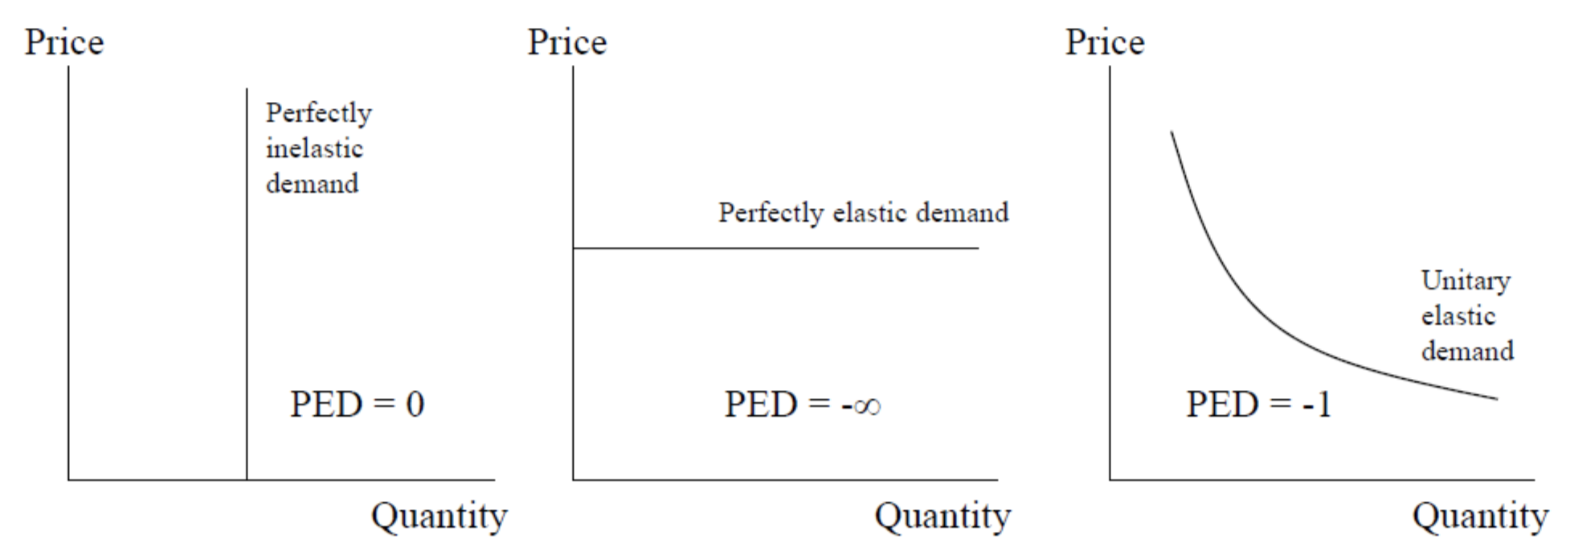
\includegraphics[width=\textwidth]{priceElasticity}
\caption{Demand curves with different values of $\epsilon^D$.}
\label{fig:difPriceElasticity}
\end{centering}
\end{figure}

\subsection{Supply}
\begin{quote}
\centering
\textbf{Supply:}\introduce{Supply} The quantity of a good or service that suppliers are willing and able to sell at any given price (in a given time period).
\end{quote}
It is usually assumed that \introduce{Link to price?} \textbf{there is a positive relationship between the price of a good and the quantity supplied of that good}. Similarly, the quantity supplied of a good is also affected by a number of different factors including: \introduce{Supply Factors}
\begin{itemize}
\item Technology
\item Costs of production inputs (e.g. labour costs, raw material costs ...)
\item Government regulation (e.g. safety regulation, taxes \& subsidies ...)
\end{itemize}
The Price Elasticity of Supply \introduce{$\epsilon^S$}, $\epsilon^S$, is \textbf{analogous to the Price Elasticity of Demand}, $\epsilon^D$ except that it is \textbf{usually positive} since increasing the price tends to increase the quantity of a good supplied.


\subsection{Market Equilibrium}
At $(Q^*, P^*)$ quantity demanded exactly equals the quantity supplied and the market is said to be in equilibrium. \introduce{Intuition?} If demand exceeds supply, buyers will bid up in accordance with either valuation of the good. If supply exceeds demand, suppliers will attempt to undercut prices in order to sell their product.

$\epsilon^D$ \& $\epsilon^S $ are very important when assessing the affects of shifts in supply and demand; a shift in demand may mostly increase the quantity or the price depending on whether supply is elastic or inelastic.

\begin{figure}[H]
\begin{centering}
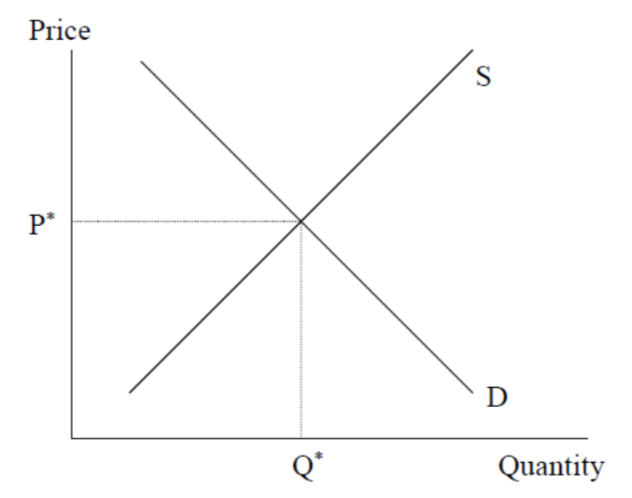
\includegraphics[width=0.4\textwidth]{marketEquilibrium}
\caption{Market Equilibrium}
\label{fig:marketEquilibrium}
\end{centering}
\end{figure}

\subsection{Price Controls}
There are two main types of price controls.

Price Ceilings \introduce{Price Ceilings} place a maximum price for the good below the equilibrium price for buyer benefit e.g. rent controls. This results in a supply shortage which requires some form of rationing.

\begin{figure}[H]
\begin{centering}
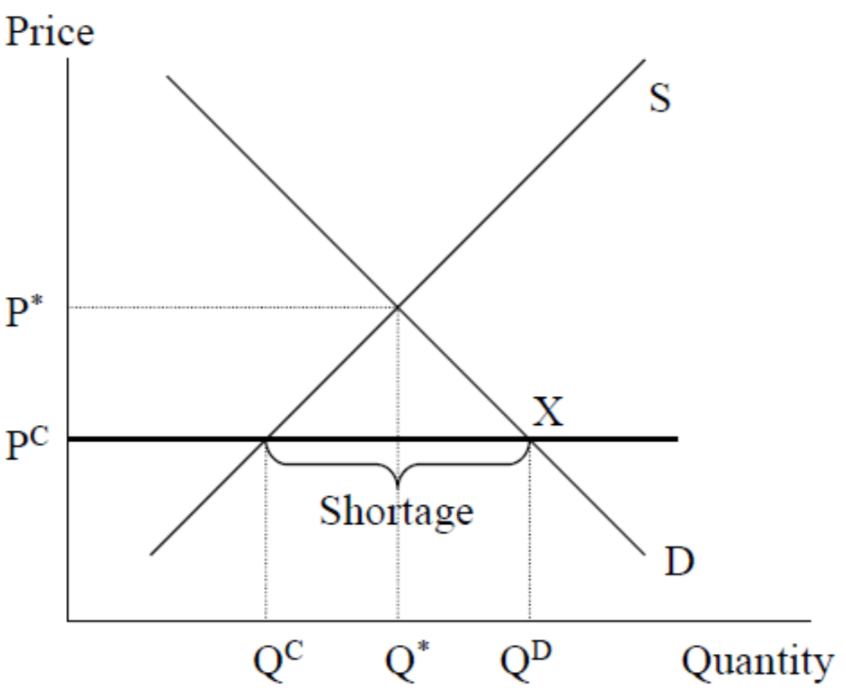
\includegraphics[width=0.4\textwidth]{priceCeiling}
\caption{A Price Ceiling. In effect, the demand curve is the line $P^CXD$.}
\label{fig:priceCeiling}
\end{centering}
\end{figure}

Price Floors \introduce{Price Floors} place a minimum price for the good above the equilibrium price for seller benefit e.g. minimum wage. This results in a supply surplus which may result in the Government purchasing the excess.

\begin{figure}[H]
\begin{centering}
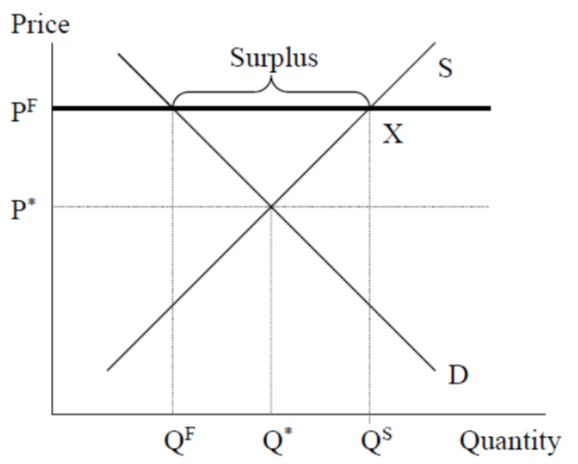
\includegraphics[width=0.4\textwidth]{priceFloor}
\caption{A Price Floor. In effect, the supply curve is the line $P^FXS$.}
\label{fig:priceFlor}
\end{centering}
\end{figure}

\section{The Consumer}
\subsection{The Rational Agent Model}
It is assumed that each consumer acts as a \textbf{rational agent} \introduce{The Rational Agent Model} defined by their tastes (preferences over consumption bundles) and their opportunities (the consumptions bundles which a consumer can afford). Each consumer \textbf{chooses a particular consumption bundle}, $\boldsymbol{x} \in \mathbb{R}^n_+$ where $\boldsymbol{x} = (x_1, x_2, ..., x_n)$. Each $x_i$ denotes the amount of good $i$ in the bundle and is assumed to be non-negative and perfectly divisible. The following axioms \introduce{Axioms} are imposed upon rational consumers, denoting $\mathcal{X}$ as the space of all consumption bundles.
\begin{enumerate}
\item \underline{Completeness} \introduce{Completeness}

\begin{quote}
\centering
For bundles $\boldsymbol{x}, \boldsymbol{y} \in \mathcal{X}$, either $\boldsymbol{x} \succeq \boldsymbol{y}$ or $\boldsymbol{y} \succeq \boldsymbol{x}$.
\end{quote}
The consumer cannot be indecisive. \introduce{Intuition}

\item \underline{Transivity} \introduce{Transitivity}

\begin{quote}
\centering
For bundles $\boldsymbol{x}, \boldsymbol{y}, \boldsymbol{z} \in \mathcal{X}$, if $\boldsymbol{x} \succeq \boldsymbol{y}$ and $\boldsymbol{y} \succeq \boldsymbol{z}$, then $\boldsymbol{x} \succeq \boldsymbol{z}$ .
\end{quote}
The consumer bundle preferences must be consistent and non-cyclic. \introduce{Intuition}

\end{enumerate}

The \introduce{Additional Assumptions} above axioms are sufficient for a consumer to be rational but economists often impose further assumptions.

\begin{enumerate}
\item \underline{Monotonicity} \introduce{Monotonicity}

\begin{quote}
\centering
For $\boldsymbol{x}, \boldsymbol{y} \in \mathcal{X}$, if $\boldsymbol{x} >> \boldsymbol{y}$ then $\boldsymbol{x} \succ \boldsymbol{y}$.
\end{quote}
More is better. \introduce{Intuition} The above is known as \textbf{weak} monotonicity; strict monotonicity states the same if $x_i \geq y_i, \boldsymbol{x}\neq\boldsymbol{y}$

\item \underline{Local Non-satiation} \introduce{Local Non-satiation}

\begin{quote}
\centering
For bundle $\boldsymbol{x} \in \mathcal{X}$ and every $\epsilon > 0$, there exists $\boldsymbol{z} \in \mathcal{X}$ such that $|\boldsymbol{z}-\boldsymbol{x}|\leq\epsilon$ and $\boldsymbol{z} \succ \boldsymbol{x}$ .
\end{quote}
The consumer can always find a local preferential bundle. \introduce{Intuition}

\item \underline{Convexity} \introduce{Convexity}

\begin{quote}
\centering
For bundles $\boldsymbol{x}, \boldsymbol{y}, \boldsymbol{z} \in \mathcal{X}$ where $\boldsymbol{x} \succeq \boldsymbol{z}$, $\boldsymbol{y} \succeq \boldsymbol{z}$ and $\boldsymbol{x} \neq \boldsymbol{y}$, for every $\alpha \in [0, 1],\ \ \ \alpha\boldsymbol{x} + (1-\alpha)\boldsymbol{y} \succeq \boldsymbol{z}$ .
\end{quote}
The consumer has a taste for variety. \introduce{Intuition} The above is known as \textbf{weak} convexity; strict convexity states that the linear combination is \textbf{strictly} preferred.

\end{enumerate}

The utility function \introduce{The Utility Function} $u: \mathcal{X} \rightarrow \mathbb{R}$ represents consumer preferences if for any $\boldsymbol{x}, \boldsymbol{y} \in \mathcal{X}$, $u(\boldsymbol{x}) \geq u(\boldsymbol{y})$ iff $\boldsymbol{x} \succeq \boldsymbol{y}$. Utility is a relative measure with meaningless absolute values and hence monotonic transformations of the utility function have no effect on the utility function.

\textbf{Indifference curves} can also be used to represent consumer preferences. \introduce{Indifference Curves} An indifference curve (IC) shows a set of bundles which a consumer is indifferent between. On an indifference curve, each point represents a different consumption bundle and the convex shape and negative slope follow from strict convexity and non-satiation \introduce{Convex?} (any linear combination of two bundles gives a preferred bundle and hence hence the curves are convex). Furthermore, \introduce{Can they cross?} transitivity implies that IC curves cannot cross; the same bundle cannot give two different utilities.

\begin{figure}[H]
\begin{centering}
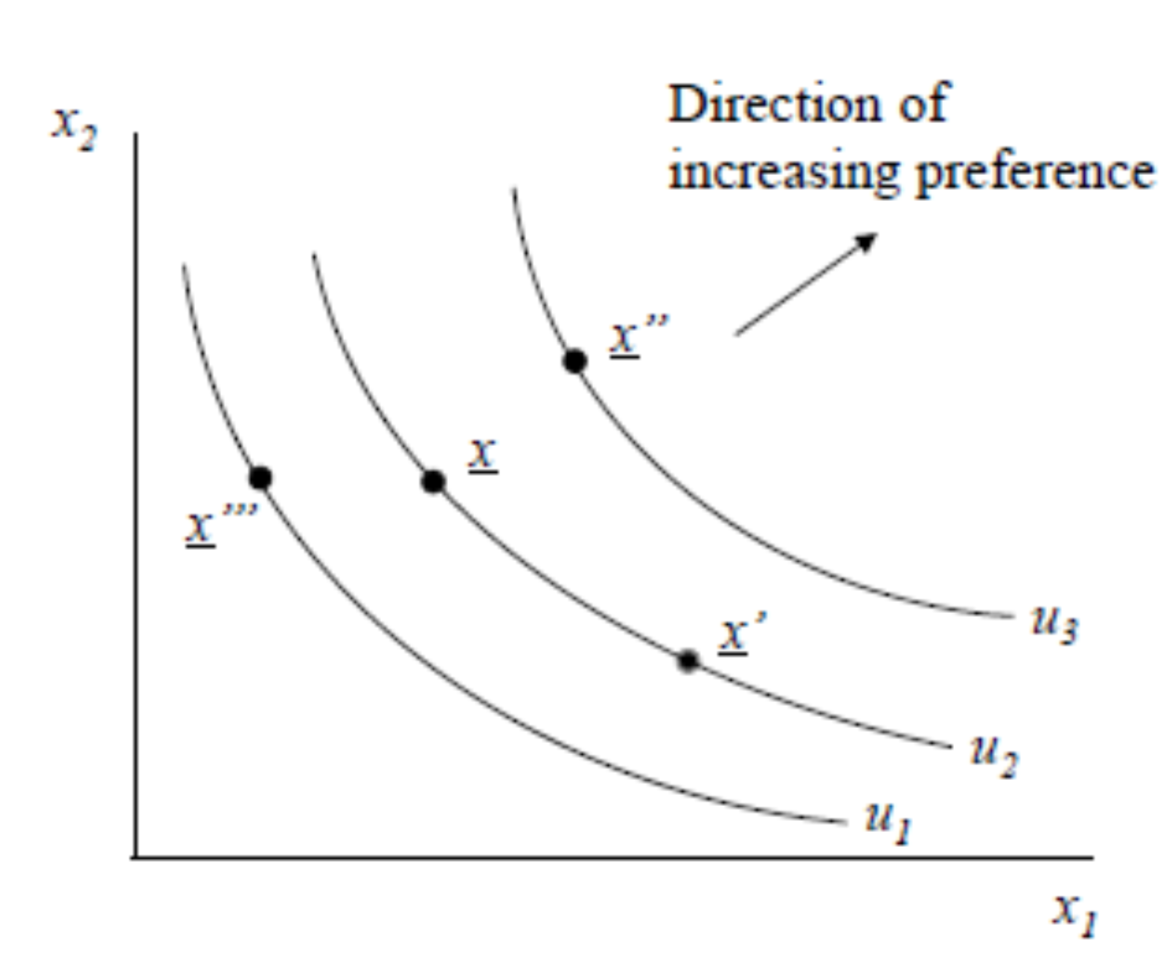
\includegraphics[width=0.4\textwidth]{indifferenceCurves}
\caption{Indifference Curves}
\label{fig:indifferenceCurves}
\end{centering}
\end{figure}

The marginal rate of substitution (MRS) \introduce{Marginal Rate of Substitution} measures the rate at which one consumer is willing to substitute a small amount of one good for another, holding utility constant and hence is the (absolute value of the) slope of an IC.

\begin{equation*}
MRS = \frac{\Delta x_2}{\Delta x_1} = \frac{\Delta u}{\Delta x_1} \frac{\Delta x_2}{\Delta u} = \frac{\partial u(x_1, x_2)/\partial x_1}{\partial u(x_1, x_2)/\partial x_2}
\end{equation*}

Goods are substitutes if as the quantity demanded for one good rises, the quantity demanded for the other good falls e.g. butter \& margarine. Two goods are perfect substitutes \introduce{Perfect Substitutes} if the MRS is constant. The utility function is a linear combination of the two goods and hence each indifference curve is a downwards sloping straight line.

Goods are complements if the quantity demanded of one good rises, the quantity demanded of the other goods also rise e.g. ice cream \& ice cream cones. Perfect complements \introduce{Perfect Complements} are goods that are always consumed together in fixed proportions. Hence $u=min(\alpha x_1, \beta x_2)$ and the indifference curves look like axis.

\begin{figure}[H]
\begin{centering}
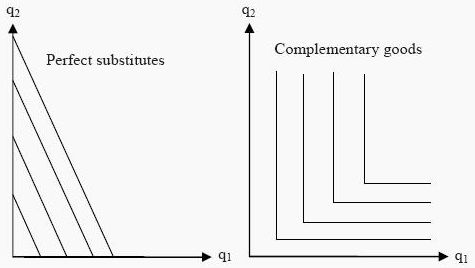
\includegraphics[width=0.4\textwidth]{complemVsSub}
\caption{Indifference Curves for perfect complements and perfect substitutes.}
\label{fig:indifferenceCurvesComplementsSubstitutes}
\end{centering}
\end{figure}

In reality, consumer opportunities are constrained by their budget. \introduce{The Budget Constraint} Consumers solve a utility maximisation problem where $p_i$ is the price of good $i$ and $M$ is the income which the consumer has available to spend.
\begin{equation*}
\boldsymbol{x} = arg\ max\ u(\boldsymbol{x})\ s.t.\ \sum_{i=1}^{N} p_ix_i \leq M
\end{equation*}
With well behaved preferences, \introduce{The solution} a tangency solution applies where the slope of the indifference curve matches the slope of the budget line and as such consumers cannot increase their utility by moving along the budget line (which they must do). However, note that there are exceptions to this such as concave indifferent curves. In general, either the tangency solution applies or a corner solution applies and it generally suffices to evaluate the utility of both.

Indifferent curves are linked to the demand curve for an individual. \introduce{Link to Demand?} If several budget lines are drawn for different $M$, the prices and quantity demanded can be extracted from the utility maximisation problem to form the demand curve for an individual.

\subsection{Types of Goods}
There are several classes of goods.
\begin{enumerate}
\item For \textbf{Normal Goods} \introduce{Normal Goods}, the quantity demanded increases as income rises.
\item For \textbf{Inferior Goods} \introduce{Inferior Goods}, the quantity demanded falls as income rises. Examples include low-quality goods such as supermarket own brand, frozen meals and canned food.
\item \textbf{Ordinary Goods} \introduce{Ordinary Goods} obey the law of demand; as their price falls, their quantity demanded rises.
\item \textbf{Giffen Goods} \introduce{Giffen Goods} do not obey the law of demand; their quantity demanded rises with price.
\end{enumerate}

\subsection{The Income \& Substitution Effects}
The effect of a change in price of a good on the quantity demanded of that good can be decomposed into two effects.
\begin{enumerate}
\item \underline{The Substitution Effect} \introduce{The Substitution Effect} \newline
The change in quantity demanded resulting from the change in \textbf{relative} prices, \textbf{holding utility constant}. This is always in the \textbf{opposite direction to the price change} i.e. a fall in price causes an increase in quantity demanded for the substitution effect.

\item \underline{The Income Effect} \introduce{The Income Effect} \newline
The change in quantity demanded resulting from the change in \textbf{purchasing power}, \textbf{holding relative prices constant}. If the good is a normal good, the income effect is in the opposite direction to the price change but if the good is an inferior good, it is in the same direction as the price change (i.e. if the price falls, the quantity demanded also falls).
\end{enumerate}
This decomposition can be illustrated graphically. \introduce{Income \& Subsitution Effects - Graphs}


\begin{figure}[H]
\begin{centering}
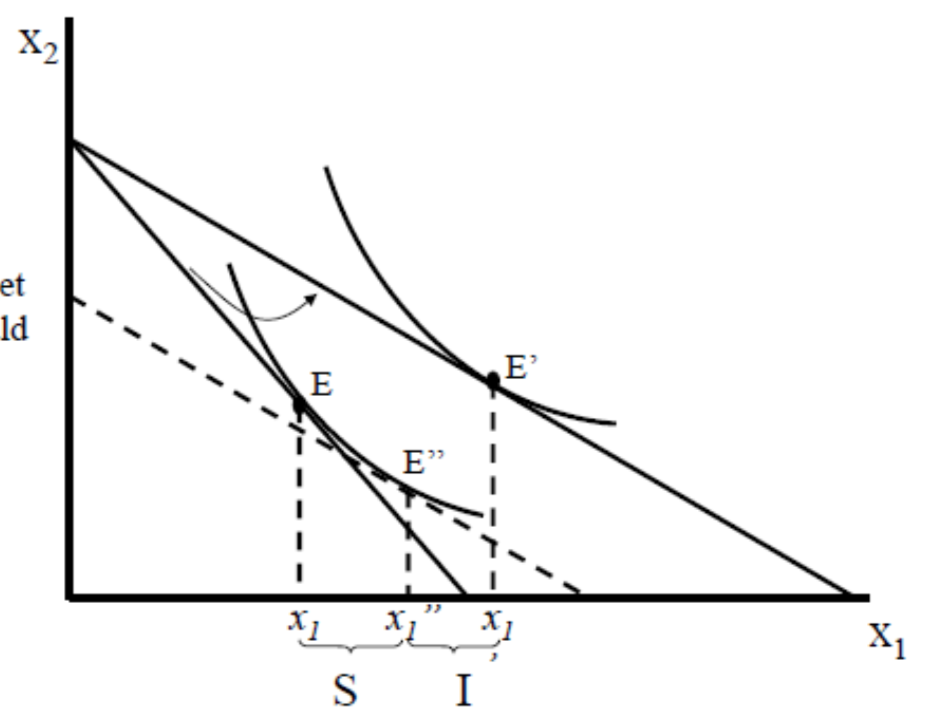
\includegraphics[width=0.5\textwidth]{incomeSubstitution}
\caption{Graphical illustration of the income \& substitution effects.}
\label{fig:incomeSubstitution.}
\end{centering}
\end{figure}

Hence Giffen Goods may be understood better;\introduce{Understanding Giffen Goods} they are \textbf{extremely inferior goods} whose \textbf{income effect outweighs the substitution effect}. It is incredibly hard to find real world examples.

\begin{figure}[H]
\begin{centering}
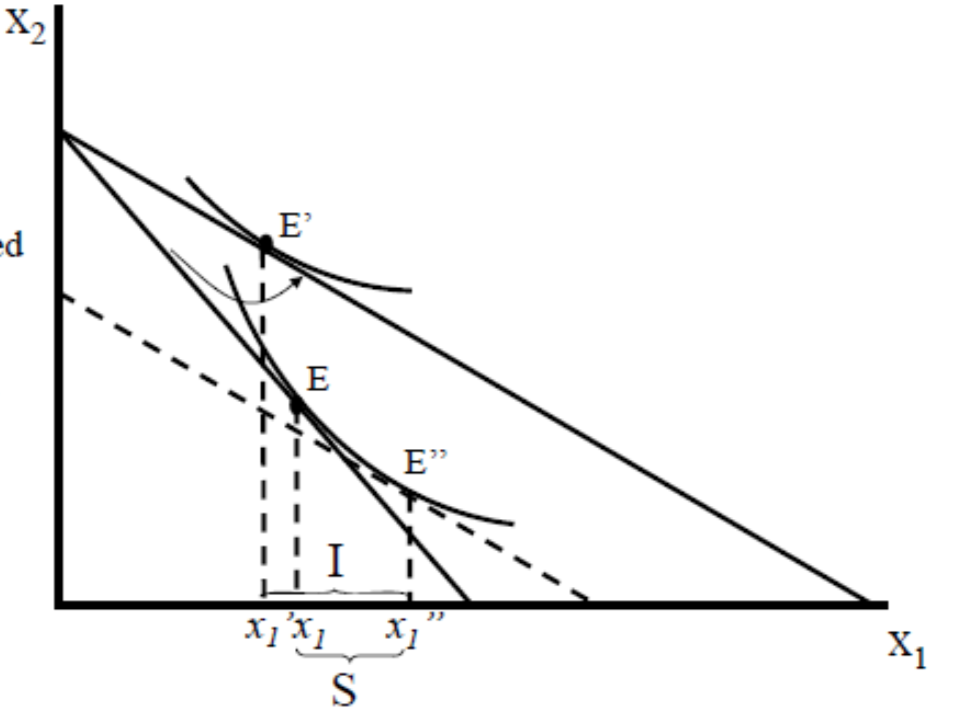
\includegraphics[width=0.5\textwidth]{giffenIndiff}
\caption{Graphical illustration of the income \& substitution effects for a Giffen good.}
\label{fig:giffenIndiff.}
\end{centering}
\end{figure}

\section{The Firm}
\subsection{The Individual}
For the purpose of analysis, we will assume that \ix{Objective} the objective of each firm is to maximise profits and disregard alternative objectives such as revenue or growth maximisation and other political objectives.

\begin{quote}
\centering
Profit ($\pi$) = Total Revenue ($TR$) - Total Cost ($TC$)
\end{quote}

The firms solves the profit maximization problem.
\begin{align*}
\max_q \pi(q) &= TR(q) - TC(q) \\
\therefore \frac{d\pi}{dq} = 0 &\Leftrightarrow MR(q) = MC(q)
\end{align*}

There are concerns with the profit maximising assumption\ix{Assumption Worries}: managerial incentives are not equivalent to ownership incentives and inefficient firms do in fact survive. However, whilst not strictly speaking true, profit maximisation serves as a useful benchmark.

Define the cost function\ix{Cost Function} $C(q)$ as the \textbf{minimum} cost of producing a given quantity, $q$. A typical cost function is $C(q) = F + VC(q)$. Note that we define the marginal cost \ix{Marginal Cost} as the cost of producing an additional unit of output, $\frac{dC}{dq}$ and the average cost, $AC$, rises if $MC>AC$. $F$, the fixed cost may be avoidable (i.e. recoverable) or sunk.

Economies of scale are important\ix{Economies of Scale}; if the slope of the $AC$ is negative there are increase returns to (or economies of) scale and if positive decreasing returns to scale. The minimum efficient scale of production (MES) \ix{MES} is the smallest output which minimizes the long-run average cost.

The short run\ix{Short Run} is defined as the period of time during which \textbf{at least} one factor of production of fixed whilst in the long run, production technology can be adapted to the market conditions.

The opportunity cost\ix{Opportunity Cost} of a product is the value of the best forgone alternative use of the resources used to make the product. Hence, when \textbf{normal profit}\ix{Normal Profit} (selling price minus opportunity cost) is negative, a firm will quit because they could have made more money elsewhere.

\section{Market Structures}
\subsection{Perfect Competition}
A perfectly competitive market\ix{Assumptions} is a market with a large number of firms each of whom is a price taker due to the large number of firms selling \textbf{homogenous goods} meaning that consumers are indifferent between stores. Consumers have perfect information and there are no transaction costs. \textbf{Crucially, there are no barriers to entry} but there are many barriers to entry in the real world, including\ix{Entry Barriers}:
\begin{itemize}
\item Government restrictions (e.g. patents).
\item Economies of scale.
\item Large sunk costs deter hit and run entry.
\item Consumer switching costs, whether that be time or otherwise.
\item Network effects: consumer utility from certain goods with depend on how many other people use it.
\end{itemize}

The profit maximisation problem reduces to $p=MC(q)$ and hence the marginal cost curve acts as the supply curve of the firm.

A firm will only remain in the market\ix{Shutdown Decisions} when the revenue from the market exceeds the costs that can be avoided by not producing. \textbf{In the short run, avoidable costs do not include sunk costs} and hence a firm will shut down if $p < AAC(q)$ where $AAC(q)$ is the average avoidable cost. \textbf{In the long run, avoidable costs include sunk costs} and hence a firm will shut down when $p < AC(q)$.

In the short run, firms are able to make profits because new firms cannot enter the market. However, in the long run there is free entry and exit and hence new firms can enter the market driving the price down to the minimum of the $AC$ curve. The long-run industry supply curve is horizontal at the minimum of the AC curve.

The perfectly competitive outcome\ix{Outcome Desirability} is highly desirable. Since $p=MC(q)$, the firm only produces an additional unit if it can cover the cost, maximising producer surplus and consumer surplus is also maximised as the value placed on the marginal good exactly equals the cost of that good; this is \textbf{consumption efficiency.} Production also occurs at the minimum average cost and no better alternative use of resources is possible; the perfectly competitive outcome is also \textbf{productively efficient.} \textbf{Pareto efficiency}\ix{Pareto Efficiency} is an allocation of resources for which it is impossible to make an individual better off without making at least one individual worse off. With convexity assumptions which rule out increasing returns to scale, it is possible to decentralize any Pareto optimal allocation into a perfectly competitive allocation by a choice of right prices and redistribution of income.

\ix{Market Diagram}
\begin{figure}[H]
\begin{centering}
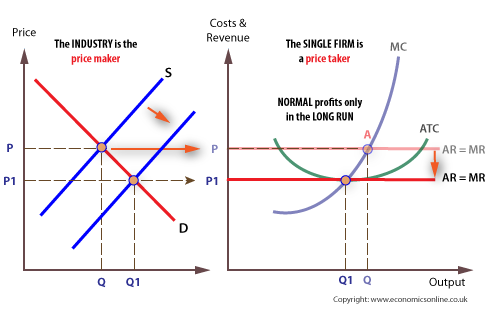
\includegraphics[width=0.7\textwidth]{perfectCompetition}
\caption{Industry and firm diagrams for perfect competition.}
\label{fig:perfectCompetition.}
\end{centering}
\end{figure}

\subsection{Monopoly}
In a monopoly, \ix{Structure}the firm is the market and hence the firm has huge market power to dictate market prices. In effect, the firm must have a price setting ability which occurs in the real world with the following examples:\ix{Price setting ability}
\begin{itemize}
\item Product differentiation.
\item Superior production technology (so other firms are unable to compete on price).
\item Government granted monopolies i.e. patents.
\end{itemize}


If the monopolist chooses quantity to maximise profits, the familiar FOC is arrived at, $MR(q)=MC(q)$. Equivalently, the monopolist could choose prices to maximise profits.
\begin{align*}
\max_p pq(p) &- C(q(p)) \\
q(p) + p\frac{dq}{dp} &= \frac{dC}{dq}\frac{dq}{dp} \\
p^{*} &= MC(q(p^*)) - \frac{q(p^{*})}{dq/dp} \\
\frac{p^{*} - MC(q(p^*))}{p^{*}} &= -\frac{1}{\epsilon(p^{*})},\ \epsilon(p) = \frac{dq}{dp}\frac{p}{q(p)} \\
p^* &= \frac{MC(q(p^*))}{1+\frac{1}{\epsilon(p^{*})}}
\end{align*}
i.e. $\epsilon(p)$ is the elasticity of demand. Considering marginal revenue for inelastic demand i.e. $-1 < \epsilon(p) < 0$, we find that the MR(q)is negative for this regions and the monopolist would never operate on this region.

Define the Lerner markup index\ix{Lerner index}, a measure of market power as.
\begin{align*}
L = \frac{p^*-MC(q(p^*))}{p^*} = \frac{-1}{\epsilon(p^{*})}
\end{align*}
Hence if the demand is more elastic there is lower markup and less market power which is intuitive. However, to quantity the loss of social welfare we compare consumer and producer surplus at the monopoly to price to the perfectively competitive outcome which does not necessarily decrease with the elasticity of demand.

\ix{Market Diagram}
\begin{figure}[H]
\begin{centering}
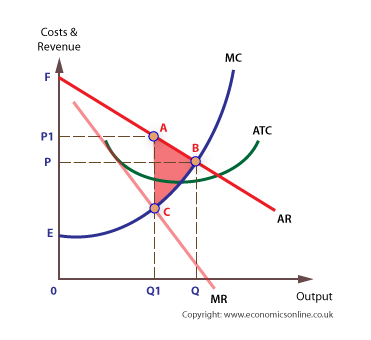
\includegraphics[width=0.5\textwidth]{monopolyWelfareLoss}
\caption{Market curve for monopoly, shaded region denotes the deadweight loss. The monopolist sells at a lower quantity because this increases the price and profits.}
\label{fig:monopoly}
\end{centering}
\end{figure}

It isn't all bad with monopoly. \ix{Playing devils advocate}Some may argue that a monopoly deserves market leadership with the lowest-cost technology or that monopoly profits provide incentive for innovation and technology change. In other cases, only large firms are truly take advantage of economies of scale. These industries are known as natural monopolies\ix{Natural Monopoly} and examples include railways. The government play a key role here to balance the amount of market competition and they regulate market power.

There are also alternatives to the Lerner index to measuring market power\ix{Measuring Market Power} which include measuring the market share (but Apple has great power over their own customers but a small share), availability of substitutes (but see the cellophane fallacy). Direct measures are given by estimating the demand elasticity.

\subsection{Oligopoly}
An oligopolist market is made up of a small number of firms and hence each firm has some, but not total, market power. There is significant strategic interaction modelled through game theory.

\subsubsection*{Cournot Model}
In the cournot model, each firm \textbf{sets the quantity which they produce}\ix{Cournot Model}.

Each firms can form a best response function given the quantity which the other firm produces (by applying the FOC). The Nash equilibrium is given by the quantities where the two best response functions intersect (i.e. plotting $q_1, q_2$) i.e. each firm is responding best to the other. Otherwise, firms will have an incentive to alter quantity of production. An expression for the Lerner index can be found and it is proportional to the firms market share.

In this model, each firm is able to make\ix{Profits?} abnormal profits. Note that if each firm did cooperate, they would be able to make larger profits but the Nash equilibrium position would not be satisfied.

Define $\alpha_i = \frac{q_i}{Q}$. The Herfindahl index, $H = \sum_i \alpha_i^2$, \ix{Herfindahl Index} is a common measure of market power with higher values indicating higher market power. More concentrated markets will have larger departures from the marginal cost but not necessarily lower welfare; welfare may be enhanced with large, low cost firms.

\subsubsection*{Bertrand Model}
In the Bertrand model\ix{Bertrand}, each firm sets their own prices. Assuming identical/homogeneous products, \textbf{all consumers will go to the firm with the lower price} and hence the best response is as follows:
\begin{align*}
BR_1(p_2) = \begin{cases}
p_2 - \epsilon\ &if p_2 - \epsilon > MC \\
MC &\text{otherwise}
\end{cases}
\end{align*}
\textbf{Effectively, firms seek to undercut each other and the price is driven down to the marginal cost, c} as which point firms can no longer reduce their prices. This is the \textbf{Bertrand paradox!} i.e. when goods are homogenous, firms act like price takers.

The Bertrand paradox\ix{Resolving the Paradox} may be resolved by noting that a firm may not be able to supply the whole market, that products are in fact not homogenous and consumer has search costs.

\subsubsection*{Collusion}
\ix{See the section on Game Theory}Collusion can be explicit where firms have built an agreement to reduce quantity etc but there is always an incentive to deviate and these agreements are not legally enforceable. Hence \textbf{tacit collusion is more important}\ix{Tacit} where firms act in their own self-interest and high profits are sustained through implicit threats. This can be modeled as \textbf{repeated Bertrand competition}.

The outcomes vary depending on whether the game is finite or infinite. If the game is finite,\ix{Finite vs Infinite} then that last game will be played as if it were static Bertrand and hence this would be anticipated and a competitive outcome achieved. However, if the game is infinite there are other SPNE e.g. the `grim trigger strategy' i.e. collude if it is the first period or collusion has occurred in all previous rounds. It must be checked that firms are willing to `punish' when the strategy specifies it and that firms are willing to cooperate in each sub-game if there was no prior deviation. Note that \textbf{firms do not agree to anything} but rather act in self-interest.

Collusion is sustainable in infinite games\ix{When collusion sustainable?} if:
\begin{enumerate}
\item The threat of punishment is credible i.e. firms would actually be willing to punish.
\item Cooperation is profitable.
\end{enumerate}
In general, as deviation becomes more profitable collusion is more difficult to sustain but as the punishment for deviating increases, collusion becomes easier. Punishments should be sever, quick and ideally across multiple markets. There are also other factors\ix{Other Factors} including:
\begin{enumerate}
\item Firms must be able to detect deviation.
\item If there a fewer firms, collusion profits are higher.
\item Entry barriers are needed to avoid `hit and run' entry.
\end{enumerate}

\subsection{Duopoly}
\subsubsection*{Stackelberg Duopoly}
Here, duopoly is approach as a dynamic game theory problem.\ix{Setup} There are two firms of which one chooses their quantity, $q_1$ and then the second firm, observing $q_!$, chooses its own quantity. A solution approach is found as follows:
\begin{enumerate}
\item Find optimal $q_2$ for all possible $q_1$. If the second firm is rational, firm 1 is able to predict their quantity.
\item With firm 1 anticipating the second firm's reaction, choose $q_1$ to maximize profits i.e. $q_1^*$ is not the best response to $q_2^*$ but rather the best response to $q_2^*(q_1)$.
\end{enumerate}
The outcome is different to the cournot situation, even if each firm is identical. Hence\ix{Order of Moves} it is clear that \textbf{the order of moves matters} and firm 1 has a first-mover advantage. Note that irreversibility is crucial; if a firm 1 is able to change it's decision having observed $q_2$, game dynamics change.

\section{Price Discrimination}
We have assumed that firms set one uniform price\ix{What is Price Discrimination?} but this is often not the case. Firms not only charge customers different prices for the same product (e.g. student discounts) but also can charge different amounts depending on the quantity purchases.

\subsection{First Degree Price Discrimination}
First degree PD\ix{First Degree PD} is when each consumer is charged exactly their willingness to pay; the seller is said to \emph{march down the demand curve}. A monopolist under this scheme will produce at $q$ where $MC(q)=MR(q)$ but will take \textbf{much higher profits} since also consumer surplus is extracted which provides the motive for this type of price discrimination.A key requirement for this type of price discrimination\ix{Requirement} is that consumers cannot trade with each other(no resale condition); otherwise the marginal customer would buy for the whole market. Furthermore, the \textbf{monopoly must know the `willingness to pay of each consumer'}.

An equivalent strategy is to\ix{Equivalently...} offer a two-part tariff where each consumer pays a fixed fee for the right to purchase and a per-unit price where $p=MC$ \& $F=CS$ i.e. the fixed cost exists to extract all consumer surplus.

\subsection{Second Degree Price Discrimination}
Here the monopoly charges a different\ix{Second Degree PD} price depending on the characteristics of the purchases e.g. quantity discounts, quality differentiation. It is assumed that \textbf{the monopolist is unable to classify consumers into groups} and hence the scheme design allows `self-selection'.

Prices are chosen according to constraints\ix{Constraints}. Assume two types of consumers, $A$ \& $B$. Denote $u_T(x)$ as the utility of good $x$ for type $T$ and $g_T$ as the good `intended' for type $T$.
\begin{enumerate}
\item \underline{Self-Selection Constraints:} Each type must prefer their allocated product.
\begin{align*}
u_A(g_A) - p_{g_A} &\geq u_A(g_B) - p_{g_B} \\
u_B(g_B) - p_{g_B} &\geq u_B(g_A) - p_{g_A}
\end{align*}
\item \underline{Participation Constraints:} Each type must prefer to purchase their good over not purchasing.
\begin{align*}
u_A(g_A) - p_{g_A} \geq 0 \hspace{1cm} u_B(g_B) - p_{g_b} \geq 0
\end{align*}
\end{enumerate}
The solution to these constraints usually results in charging one type their utility (and hence receive no net utility) and the second type the upper bound to ensure that they are indifferent between each good\ix{In words...} i.e. \textbf{make the `low type' indifferent between buying or not and the `high type' indifferent between the `high' and `low' products.}

\subsubsection*{Non-Linear Pricing}
Non-linear pricing is\ix{Non-Linear Pricing} when a consumer's expenditure doesn't rise linearly with the amount purchased. Consumers receive utility $U(q, \theta)=\theta V(q) - T(q)$ if they purchase quantity q where $\theta$ represents the consumer `type'. It is assumed that $\frac{\partial^2U}{\partial q\partial\theta}>0$ (single-crossing property\ix{Single-Crossing Property}) which implies that marginal utility of consumption increases with type. As before, the pricing is constrained. Assume two types of consumers, $A$ \& $B$. Denote $u_T(x)$ as the utility of good $x$ for type $T$ and $g_T$ as the good `intended' for type $T$.
\begin{enumerate}
\item \underline{Individual Rationality:} Each type must be willing to buy.
\begin{align*}
\theta_TV(q_T) - T_{g_T} > 0
\end{align*}
\item \underline{Inventive Compatibility:} Each type must prefer to purchase their good over other types of goods.
\begin{align*}
u_T(g_T) - p_{g_T} &\geq u_{T}(g_{T'}) - p_{g_{T'}},\ \forall T'\neq T
\end{align*}
\end{enumerate}
The\ix{Simplification} individual rationality constraints for all types which are not the lowest type are slack and the incentive compatibility constraint is slack for the lowest type.\ix{Intuition} Middle type consumers gain more from pretending to be low-type than high-type (single-crossing property; high types will gain more utility from the same quantity) and if the higher type would prefer to reveal themselves over pretending to be a middle type, then they would also prefer over pretending to be a low type.

All consumer surplus can be extracted\ix{Outcomes} from the lowest type but higher type consumers are left with surplus since they could always buy the lowest type bundle and obtain net-surplus. There is \textbf{no distortion at the top} where marginal utility equals costs whilst the consumption of the `lower' consumers is distorted downwards. The outcomes can be summarised as follows:
\begin{itemize}
\item Higher types receive higher quantities (or higher quality).
\item No rents for the low type; they receive zero utility.
\item Information rents for the high types who could always have net-utility with the low type product.
\item Efficiency at the top where $\theta_HV'(q_H)=c$ whilst there is distortion at the bottom where $\theta_LV'(q_L)>c$.
\item Quantity discounts.
\end{itemize}

The monopolist may not want to sell to the lower types if their proportion is too low\ix{Why sell to the lower types?}; recall that it is the higher-types that make net-surplus.

Outside options are important;\ix{Outside options} in the case where each type has different outside options denoted as $u_T$, purchasing must be preferred to the outside options and hence if $u_H > u_L$ then the lower types want to mimic high types and it is no longer obvious which constraints are binding.



\subsection{Third Degree Price Discrimination}
It is assumed\ix{Assumptions} that the monopolist knows the demand functions for different groups of consumers which differ in their price responsiveness. The monopolist is also assumed to be unable to distinguish between consumers in each group. The monopolist charges a different, profit maximising price to each group following the \ix{Inverse Elasticity Rule: Again?}inverse elasticity rule; consumers who are less-elastic will be charged higher prices.

Third degree price discrimination\ix{Effects} affects the distribution of income as different groups are charged different prices. The monopolist will \textbf{always make higher profits in this regime} as there is no incentive to otherwise. \textbf{The consumer surplus may rise} if the total output rises but this is problem dependent.

Similarly, there is an equivalent two part tariff for this form of price discrimination, extracting all consumer surplus.

\subsection{Indirect Price Discrimination}
Often goods are sold together as a package, for example, a CD contains many songs.\ix{Bundling} Pure bundling is when goods are available only as part of a bundle whilst mixed bundling allows for individual sales. If preferences are negatively correlated, there are different high-buyers for each good and bundling can act as a form of price discrimination, as if each firm was paying a different price for each good. If products are `extremely' negatively correlated the firm will maximize profits by only selling products to one customer.

\ix{Tie-In Sales}Firms also often sell two complementary products where ownership of one good is a requirement for consumption of the other.

\section{Game Theory}
A game is a model of strategic decision making and hence this section is very heavily linked to oligopoly.

\subsection{Static Games of Complete Information}
Games in which\ix{Static Games of Complete Information} each players choose their strategies simultaneously (static) and receive payoffs depending on the strategies chosen (a game) are said to have complete information if each player's payoff function is common knowledge amongst all players.

We can describe a game using the \emph{normal form representation}\ix{Normal Form}. Specify:
\begin{enumerate}
\item Players $i \in N = \lbrace 1, \ldots, n\rbrace$.
\item The strategies available to each player $s_i \in S_i$.
\item The payoff received by each player for a combination of strategies $u_i(s_i, \ldots, s_n)$
\end{enumerate}
Hence the normal form representation of an $n$ player game, G, is $G = \lbrace S_1, \ldots, S_n; u_1, \ldots, u_n \rbrace$. A game is said to be zero-sum is the sum of the payoffs in each outcome is zero.

A \textbf{strictly}\ix{Strictly Dominant Strategies} \textbf{dominant strategy} for player $i$ gives strictly higher payoffs than any other available strategies, regardless of what the other players do.

A (strictly)\ix{Strictly Dominated Strategies} \textbf{dominated strategy} for player $i$ gives strictly lower payoffs than \textbf{any other} available strategy, regardless of what the other players do (i.e. the player has another strategy which leads to strictly higher payoffs).

A player's\ix{Best Response Strategy} \textbf{best response strategy} gives the optimal move(s) that should be taken in response to a set of strategies played by all other players. i.e.
\begin{align*}
S_{/i}^{n} &= \lbrace s_1,..., s_{i-1}, s_{i+1}, ..., s_n \rbrace \\
s_i \in BR(S_{/i}^{n}) &\Leftrightarrow u_i(s_i, S_{/i}^{n}) \geq u_i(s_{i}^\prime, S_{/i}^{n})\ \forall s_{i}^\prime \in S_i
\end{align*}

A mixed strategy\ix{Mixed Strategies} for a player $i$ is a probability distribution over the pure strategies in $S_i$

\subsubsection*{Solution Concepts}
There are several solution concepts which can be used to `solve' games.
\begin{enumerate}
\item \underline{Dominant Strategies}

If players have dominant strategies, they will play them. However, players may not have dominant strategies.

\item \underline{Iterated Deletion of Dominated Strategies}

Players may have dominated strategies but not dominant strategies. Since \textbf{A rational player can only play undominated strategies} since a better outcome can always be achieved, repeatedly deleting dominated strategies (since there is complete information, other players also know that they will never play these strategies) can lead to a solution, assuming rationality.

\item \underline{Nash Equilibrium}

A\ix{Nash Equilibrium} Nash equilibrium is a profile of strategies such that each player's strategy is the best response to the other players' strategies.

A strategy profile $s^* = \lbrace s_1^*, ..., s_n^*\rbrace$ is a \emph{Nash Equilibrium} of a game, $G = \lbrace S_1, \ldots, S_n; u_1, \ldots, u_n \rbrace$ if
\begin{align*}
\forall i: s_i^* \in BR(S^n_{/i})
\end{align*}
i.e. each player is playing their own best response strategy. \textbf{There are usually an odd number of Nash equilibrium} in which case the theory does not predict which equilibrium is chosen.
\end{enumerate}

If an even number of pure Nash equilibria have been found, it is likely that there is a Nash equilibrium in mixed strategies\ix{Mixed Equilibria}. For a two player game, the expected payoff is
\begin{align*}
v_i(P_1, P_2) = \sum_j \sum_k p_{1j} p_{2k} u_i(s_{1j}, s_{2k})
\end{align*}
Denoting $\Delta S_i$ as the set of all probability distributions over $S_i$, $(P_1^*, P_2^*)$ is a Nash Equilibrium of the game $G = \lbrace \Delta S_1, \Delta S_2; u_1, u_2\rbrace$ iff each player's mixed strategy is a best response to the other player's equilibrium strategy. i.e.
\begin{align*}
v_1(P_1^*, P_2^*) &\geq v_1(P_1, P_2^*)\ \forall P_1 \in \Delta S_2 \ \ \ \text{and} \\
v_2(P_1^*, P_2^*) &\geq v_1(P_1^*, P_2)\ \forall P_2 \in \Delta S_2
\end{align*}
\textbf{Each player chooses their own strategy to make their rival indifferent}\ix{Indifferent Condition}. The probabilities may be interpreted as one player's beliefs about another players play.

\subsection{Dynamic Games}
Dynamic games are games in which there are multiple stages and decisions may not be made simultaneously. When writing in normal form, often find \textbf{non-credible threats} as Nash equilibria which rational players would not actually play (the game is really sequential) i.e. there is non-optimal behaviour in the original player plays differently.   Alternatively, \ix{Alternative} extensive form is used which accounts for the timing of game.

A sub-game-perfect Nash equilibrium \ix{SPNE} is a profile of strategies such that at \textbf{every decision node} the specified action is optimal for the player making the decision, assuming optimal decisions at all subsequent nodes. Dynamic games are solved by \textbf{backward induction} i.e. start at the last sub-game and work backwards.

There is significant strategic value to commitment.\ix{Commitment} Crucial in Stackelberg duopoly, other examples include burning bridges (e.g. `never negotiate with terrorists'). This leads to first-mover advantages if strategies are substitutes but if strategies are complements then there can be a first-mover disadvantage

\subsection{Repeated Games}
Repeated games\ix{Repeated Games} can be thought of as static games which are simply played several times with \textbf{future payoffs discounted} by $\delta$ which can be interpreted as the probability of playing the next period or decreasing value of money.

In finite games\ix{Finite Games}, players are able to consider the last game played and solve this e.g. using a dominant strategy. Then in previous periods, assuming rationality, the behaviour in the final period is anticipated and hence for finitely repeated games, a SPNE can be the normal Nash equilibrium in any one period (e.g. consider repeated prisoners dilemma).

In infinite games, define the super-game as the infinitely long game and the stage-game as the static game repeated each period\ix{Super and Stage games}. Infinitely repeated games can have several SPNE such as the `grim trigger' strategy but note that the `future' must be valued enough i.e. there is a lower bound on $\delta$. To check whether strategies are SPNE, the \textbf{one-shot deviation principle} is used. \ix{One-shot Deviation Principle}
\begin{enumerate}
\item If there is no profitable one-shot deviation from the strategy, then there is no profitable finite sequence of deviations.
\item If there is no profitable finite deviation, then there is no profitable infinite sequence of deviations.
\end{enumerate}
Hence it is enough to check whether one deviation is profitable or not.

\textbf{Folk Theorem:}\ix{Folk Theorem} Let $\pi_i^*$ denote player $i$'s payoff in the unique NE of the stage game. In the infinitely repeated game, for any feasible payoff $\hat{\pi_i} > \pi_i^*$ for every player, there exists some discount factor $0 < \hat{\delta} < 1$ such that if $\delta > \hat{\delta}$, $\hat{\pi_i}$ can be obtained as the average per-period payoff in a SPNE. This has no predictive power, simply states that there is some SPNE but not what it is.

\section{Macroeconomics}
\subsection{Premilinaries}
In an economy, national income is made\ix{National Income} up of the following components:
\begin{align*}
  Y \equiv C + I + G\ (-T_e) + NX
\end{align*}
Where $Y$ is income, $C$ is consumption, $I$ is investment, $G$ is government spending and indirect taxes (taxes levied on expenditure), $T_e$, are only included at basic prices. $NX$ are the net exports. 

Disposable income at basic prices is income\ix{Savings and $Y_d$} add transfer payments, $B$, less direct taxes (levied on sources of income), $T_d$. Savings are the part of disposable income not spent on consumption. 
\begin{align*}
  Y_d \equiv Y + B - T_d \hspace{1cm} S \equiv Y_d - C
\end{align*}

A \textbf{stock is a quantity measured at a point in time while a flow is measured per unit of time}.\ix{Stocks vs. Flows}

It is\ix{Sticky Prices} often assumed that prices are flexible and adjust to equate supply and demand. However, in the short run prices are \textbf{sticky} and adjust slowly in responses to changes in supply and demand. For example, many labour contracts fit the nominal wage for a year or longer.  The behaviour of an economy is heavily dependent upon the stickiness of the prices; short term stickiness can lead to unemployment and excess stocks but if prices are more flexible, economies are able to `clear'.

\ix{GDP}Gross Domestic Product is the total expenditure on domestically-produced final goods and services which is equal to the total income earned by domestically located factors of production. Income equals expenditure since every pound a buyer spends becomes income. 

With\ix{Equilibrium} a bar denoting that a quantity is fixed, equilibrium equates aggregate demand and supply. 
\begin{align*}
  \underbrace{C(\bar{Y} - \bar{T}) + I(r) + \bar{G} + \bar{NX}}_{\text{Aggregate Demand}} = \underbrace{F(\bar{K}, \bar{L})}_{\text{Aggregate Supply}} \text{i.e. fixed technology and labour}
\end{align*}
Hence the \textbf{real interest rate} (inflation adjusted) changes in order equate supply and demand.

\subsection{Consumption}
\ix{Definition}
\begin{quote}
\centering
Consumption is the value of all goods and services bought by households including durable, non-durable goods and services.
\end{quote}
Consumption is the largest component of aggregate demand and accounts for \(90\% \) of disposable income; hence consumption is vital for economic growth. 

Most of the theories below will imply that consumption does not vary as much as income and consumption is mostly driven by permanent income changes. Expectations of future income will also change spending patterns today and savings will be lower when future income is expected to be higher. Note that savings can be negative (i.e. borrowing) and most of the following theories rely on the ability to borrow. If borrowing is impossible, there will be higher savings. 

\subsubsection*{Keynesian Consumption}
Keynes thought that consumption was a function of \textbf{disposable income}. \ix{The Consumption Function}
\begin{figure}[H]
\begin{center}
  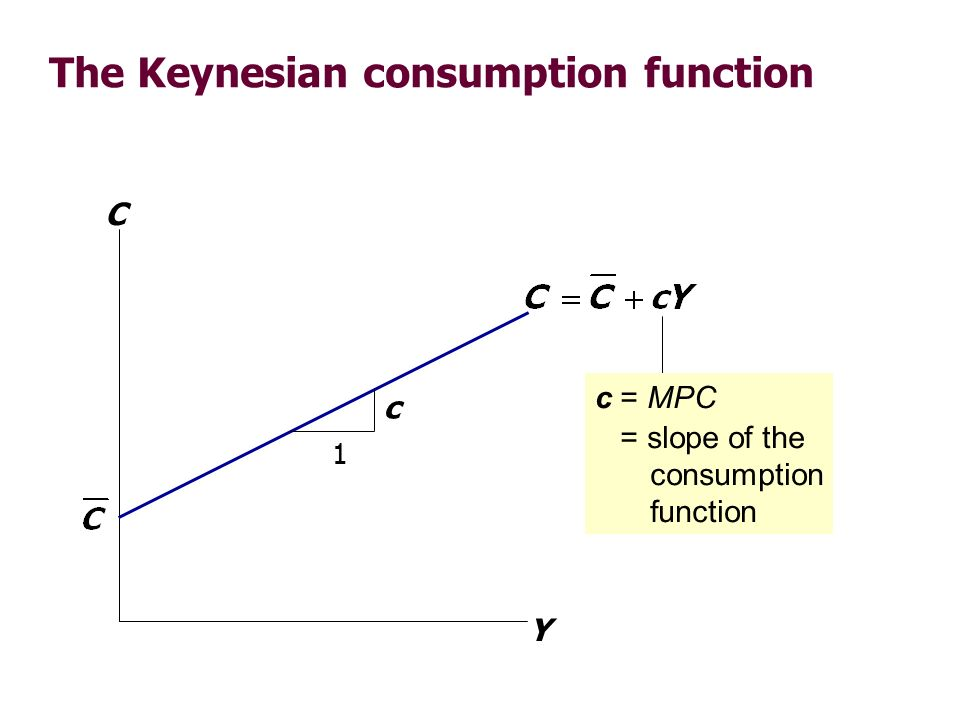
\includegraphics[width=0.6\textwidth]{keynesConsumption}
  \caption{Note: x axis should read $Y_d$. }
\end{center}
\end{figure}
The $MPC$ is in the range $(0, 1)$ and the average propensity to consume $APC = C/Y$ falls as income rises as consumers save a bigger fraction of their income. (Note the $APC$ for a given value of $C$ is the slope of a line through the origin to that point.)

This model implies\ix{Implications} that the distribution of income will affect the total consumption and that economies may suffer from `under-consumption' as they grow meaning the Government may be forced to use fiscal policy. 

Whilst this model fits short run trends since higher income \ix{Intial Findings?}households consume more, save more and save a larger fraction of their income. Income does indeed seem to be the main determinant of consumption. 

However,\ix{Problems} using this model it is predicted that $C$ should grow more slowly that $Y$ over time but in fact over time the $APC$ did not fall and $C$ grew at the same rate as income. The puzzle is that over a long period of time, the $APC$ is constant but across different households the $APC$ falls with income. 

\subsubsection*{Intertemporal Choice}
Keynes assumed that current consumption depends only on current income. However, it can be assumed that the consumer is forward looking and chooses consumption to maximise \emph{lifetime utility}. It was suggested that current consumption depends only on the present value of lifetime income and the timing of income is irrelevant as the consumer can borrow or lend between periods. 

\subsubsection*{The Life-Cycle Hypothesis}
The life cycle \ix{Premise \& Assumptions} hypothesis states that the consumer achieves smooth consumption through saving even though income varies systematically over the phases of a consumers life. For simplicity, there is assumed to be zero interest rate and consumption smoothing is optimal. 
\begin{align*}
  C = \frac{W+RY}{T}& = \alpha W + \beta Y \\
  APC &= \alpha \frac{W}{Y} + \beta
\end{align*}
where $W$ is wealth, $R$ is the time until retirement, $T$ is the lifetime and $Y$ is the income until retirement. 

The LCH can solve the consumption puzzle.\ix{Solving the Consumption Puzzle}. Across households, income varies more than wealth and so higher income households have a lower $APC$ but over time, wealth and income grow together causing the $APC$ to remain stable. 

\begin{figure}[H]
  \begin{center}
    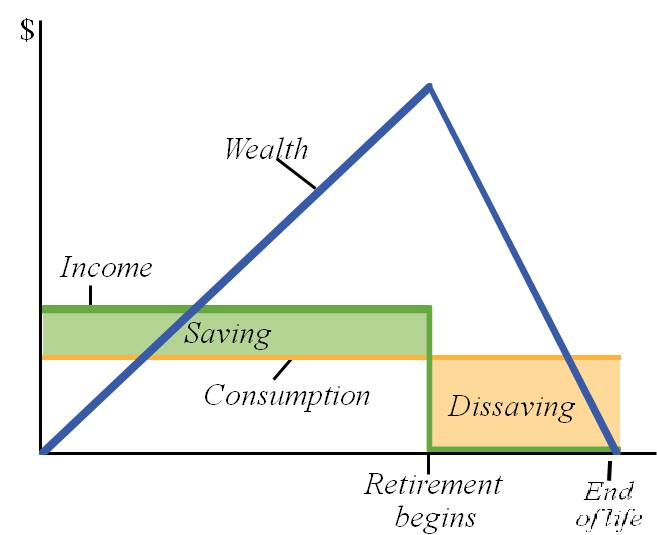
\includegraphics[width=0.4\textwidth]{lifecycle}
    \caption{The Life-Cycle Hypothesis}
  \end{center}
\end{figure}

\subsubsection*{The Permanent Income Hypothesis}
Income is split into two parts:
\begin{itemize}
  \item\ix{Permanent}Permanent income is average income expected to persist into the future e.g. salary.
  \item\ix{Transitory}Transitory income is temporary deviations from the average income e.g. inheritance, lottery winnings etc.
\end{itemize}
Consumers use saving and borrowing to smooth consumption and it is suggested that a fraction of permanent income is consumed i.e. $C=aY^P$. \ix{Solving The Consumption Puzzle} The consumption puzzle can be solved; if high income households have higher transitory income (somewhat plausible - rich are more likely to invest), the $APC$ is lower in high-income households but over the long run, income variation is due to variation in permanent income which would imply a stable $APC$.

\subsubsection*{The Random-Walk Hypothesis}
Based on the intertemporal choice and assuming rational expectations (i.e. people use all available information to forecast future variables), the random-walk hypothesis\ix{What does the model suggest?} suggests that consumption should follow be a random walk i.e. changes in income should be unpredictable.

Anticipated changes of income or wealth should already have been factored into the expected permanent income and hence such changes should not change consumers' consumption and only unanticipated changes in income or wealth that alter expected permanent income will change consumption.

\subsubsection*{An Alternative View: Behavioural Economics}
The above\ix{Are the assumptions valid?} models assume that consumers are rational and maximise lifetime utility. However, $76\%$ of consumers think they are not saving enough for retirement and consumers even consider themselves to be perfect decision makers. This can explained by the `pull of instant gratification'. Consider the following questions:
\begin{enumerate}
  \item Would you prefer a candy today or two candies in two weeks?
  \item Would you prefer a candy in a year or two candies in 54 weeks?
\end{enumerate}
Even though both questions are asking whether one is willing to wait two weeks for an extra piece of candy, \textbf{most do not wait in the first question but choose to wait in the second}. \ix{Time-Inconsistent Preference}This is an example of time-inconsistent preferences and can explain why many choose to consume immediately rather than delay consumption (i.e. save) and not save enough for retirement. 

\subsection{Investment}
\ix{Definition}
\begin{quote}
  \centering  
  Investment is new spending on capital goods that will allow increased production of goods and services in the future. 
\end{quote}
Investment accounts for around \(15-25\% \) of aggegrate demand and extra investment can improve the competitiveness of an economy which injects extra demand into the economy through additional exports. 

Whilst gross investment is total spending, net investment refers to gross investment less an estimate for capital consumption (replacement of depreciated goods). When net investment is positive, the capital stock of economy is rising. There are different types of investment:\ix{Types of Investment}
\begin{enumerate}
  \item Business fixed investment: spending on equipment and structure for production use.
  \item Residential investment: purchasing of new housing units. 
  \item Inventory investment: the value of the change of inventories of finished goods, materials and supplies. 
\end{enumerate}
Capital\ix{Supply Side} spending boosts the supply side of the economy and is crucial for \textbf{non-inflationary growth over time}:
\begin{itemize}
  \item There is a direct impact on the productive capacity of industries allowing greater supply of goods and services and hence also an impact upon living standards.
  \item New capital input also improve the quality of existing stock due to technological progress.
\end{itemize}

\subsubsection*{The Investment Function}
The investment function\ix{Investment Function} is \(I=I(r) \) where $r$ is the \textbf{real} interest rate (adjusted for inflation) which captures not only the cost of borrowing but also the opportunity cost of using funds to finance investment (i.e. could have put the money in the ban). Hence, $\frac{dI}{dr} < 0$.

The benefit\ix{Benefit per unit} per unit of capital is $\frac{R}{P}$ where $R$ is the nominal rate of return and $P$ is the price of the output. This is the same as the $MPK$ i.e. the marginal product of capital. 

There cost of capital is composed of a cost due to the interest rate (i.e. borrowing to spend), a cost due to the depreciation of capital and a cost due to capital losses. 
\begin{align*}
  \text{Nominal Cost of Capital }&= P_K(i + \delta + \frac{\Delta P_k}{P_k}) \\&= P_K(r + \delta) \text{  (if } \frac{\Delta P_k}{P_k} = \pi \text{ i.e. the rate of inflation)}
\end{align*}
Similarly, the above can be normalised by the price of output. The next investment depends on the profit rate from the capital. If the profit is positive, increasing $K$ is profitable but if negative the firm will increase profits by reducing the capital stock e.g. not replacing depreciated capital.

The net investment\ix{Net Investment Function} depends on the profit rate but note that total spending is net investment plus replacement of depreciated capital i.e. $\Delta K + \delta K$.
\begin{align*}
  \Delta K = I_n \Big[ MPK - \frac{P_K}{P}(r+\delta)  \Big]
\end{align*}

\begin{figure}[H]
  \begin{center}
    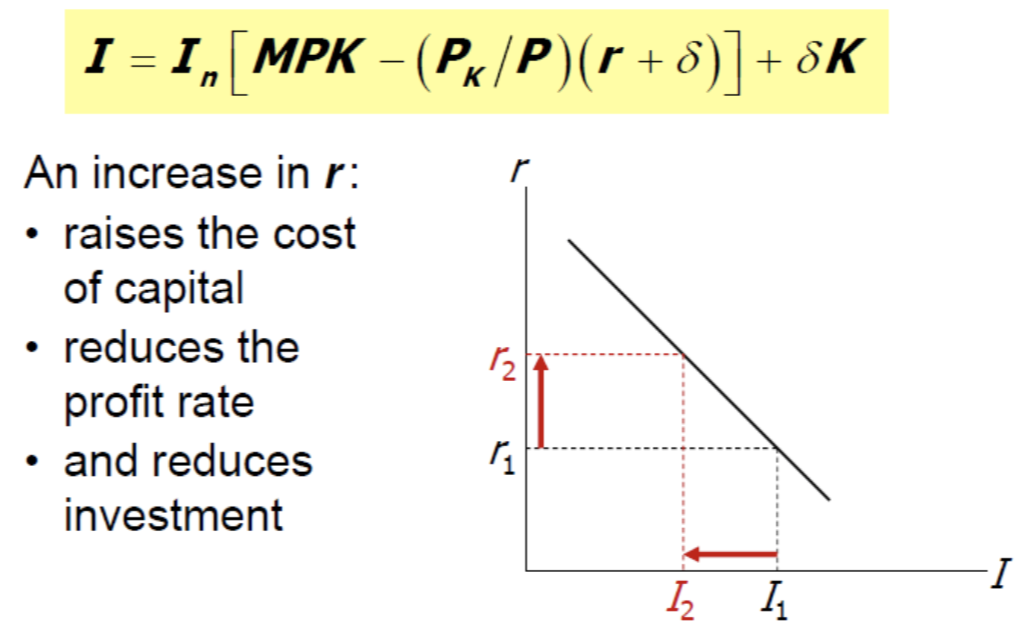
\includegraphics[width=0.6\textwidth]{investmentFunction}
    \caption{The Investment Function}
  \end{center}
\end{figure}

There are also other factors which affect investment\ix{Other Factors}:
\begin{itemize}
  \item Investment projects involve significant risk since revenue streams are uncertain, costs change over time and there is no guarantee that a project will give the required rate of return. \textbf{Changes in business confidence} can have a huge impact on investment projects and confidence is mainly driven by expectations(e.g. of demand, costs e.t.c.)
  \item Public policy can encourage investment or create uncertainty. 
  \item Technological shocks. 
  \item Quality of financial systems. 
  \item Emphasis on Stock Market dividends. 
\end{itemize}

\subsection{Government Spending}
There are several different types of government spending:\ix{Types}
\begin{itemize}
  \item Current spending: spending on goods and services for current use to directly satisfy society's needs i.e. day to day spending.
  \item Capital spending: spending on assets that create future benefits.
  \item Interest payments: payments of previously borrowed money. 
  \item Transfer payments: transfers of money as redistribution mechanisms i.e. subsidies, benefits e.t.c.
\end{itemize}
The budget balance is $G-T$ i.e. the different between government spending and tax. If in a deficit, the government must borrow to finance spending which rises to the national debt i.e the stock of outstanding government debt. If the government is `running' a surplus it can elect to reduce this debt. There is a significant link between the budget surplus and the economic cycle.

The\ix{Why tax?} government uses tax for market efficiency (e.g. correct market failure in the case of public goods) and to promote equity (a progressive tax system redistributes income from the rich to the poor). The government aims to pay for the provision of public goods but also can control aggregate demand through their fiscal policiy. There are different types of taxes:\ix{Types of Tax}
\begin{itemize}
  \item Direct taxes are levied on earnings i.e. labour, rent, dividends, interest e.t.c.
  \item Indirect taxes are levied on expenditure on goods and services i.e. VAT.
  \item Wealth taxes are taxes on capital e.g. capital transfer tax, tax on property.
\end{itemize}

\subsubsection*{Keynesian Cross}
There is a different between actual and planned expenditure and this is given by unplanned inventory investment. In equilibrium, \textbf{actual expenditure equals planned expenditure}\ix{Equilibrium}. \textbf{Note that we assume a closed economy} and that investment is assumed to be exogenous.
\begin{align*}
  PE = C(Y-\bar{T}) + \bar{I} + \bar{G}  = Y \text{ (In equilibrium)}
\end{align*}
This gives rise to the `Keynesian Cross'.

\begin{figure}[H]
  \begin{center}
    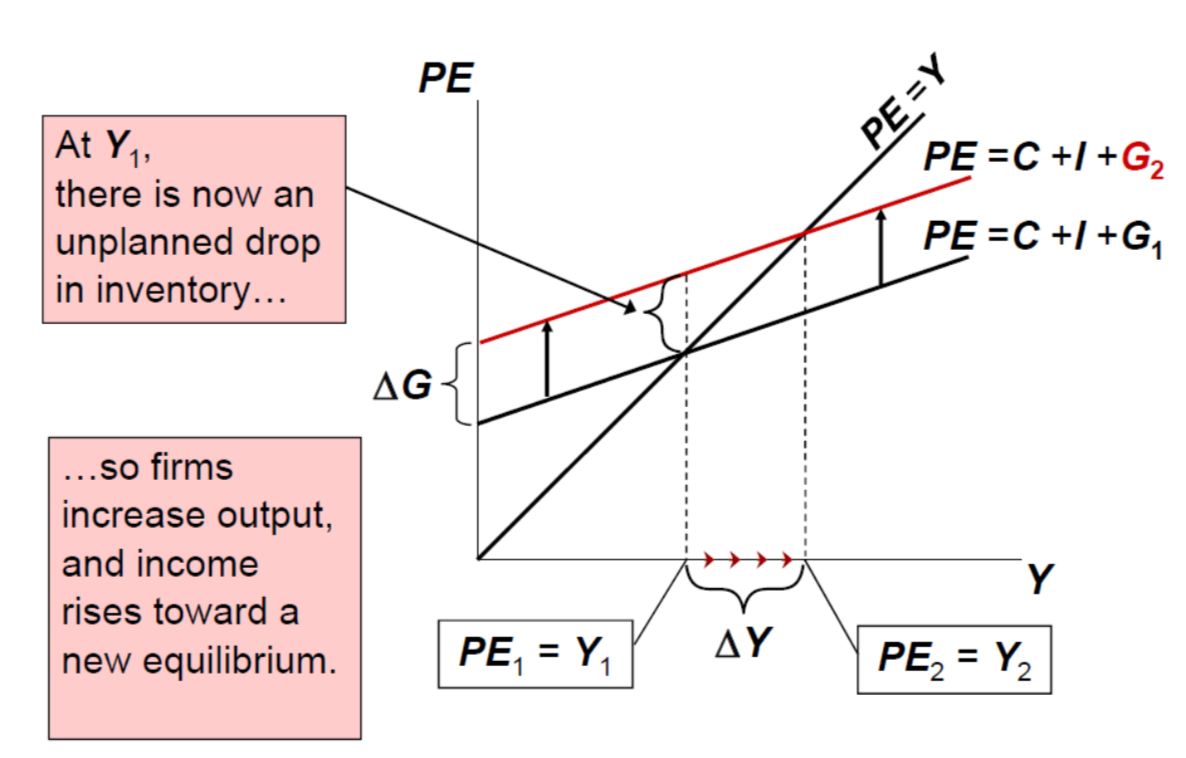
\includegraphics[width=0.6\textwidth]{keynesCross}
    \caption{The Keynesian Cross: Changing government spending.}
  \end{center}
\end{figure}

The increase of income exceeds the increase in government spending due to the\ix{Multiplier Effect} \textbf{multiplier effect}. For example, differentiating the equilibrium condition gives the following
\begin{align*}
  Y &= C(Y-\bar{T}) + \bar{I} + \bar{G} \\
  \Delta Y &= MPC\cdot \Delta Y + \Delta G \\
  \frac{\Delta Y}{\Delta G} &= \frac{1}{1 - MPC} > 1\hspace{1cm} \because MPC < 1
\end{align*}
The multiplier\ix{Intuition} exceeds $1$ as one mans income is another mans expenditure. The increase causes an equal increase in $Y$ which causes a further increase in $Y$ (since greater income causes greater expenditure) which then increases $Y$ further and so on and so forth. Since the $MPC<1$, the effect does indeed converge.

Similarly to the government spending multiplier, there is a tax multiplier.\ix{Tax Multiplier} It can be shown that
\begin{align*}
  \frac{\Delta Y}{\Delta T} = - \frac{MPC}{1-MPC}
\end{align*}
This multiplier is negative since increasing tax decreases income/output/expenditure and is smaller than the spending multiplier by a factor of the MPC (in effect, there is a smaller increase of consumption since only a proportion of the tax saving is spent).

\begin{figure}[H]
  \begin{center}
    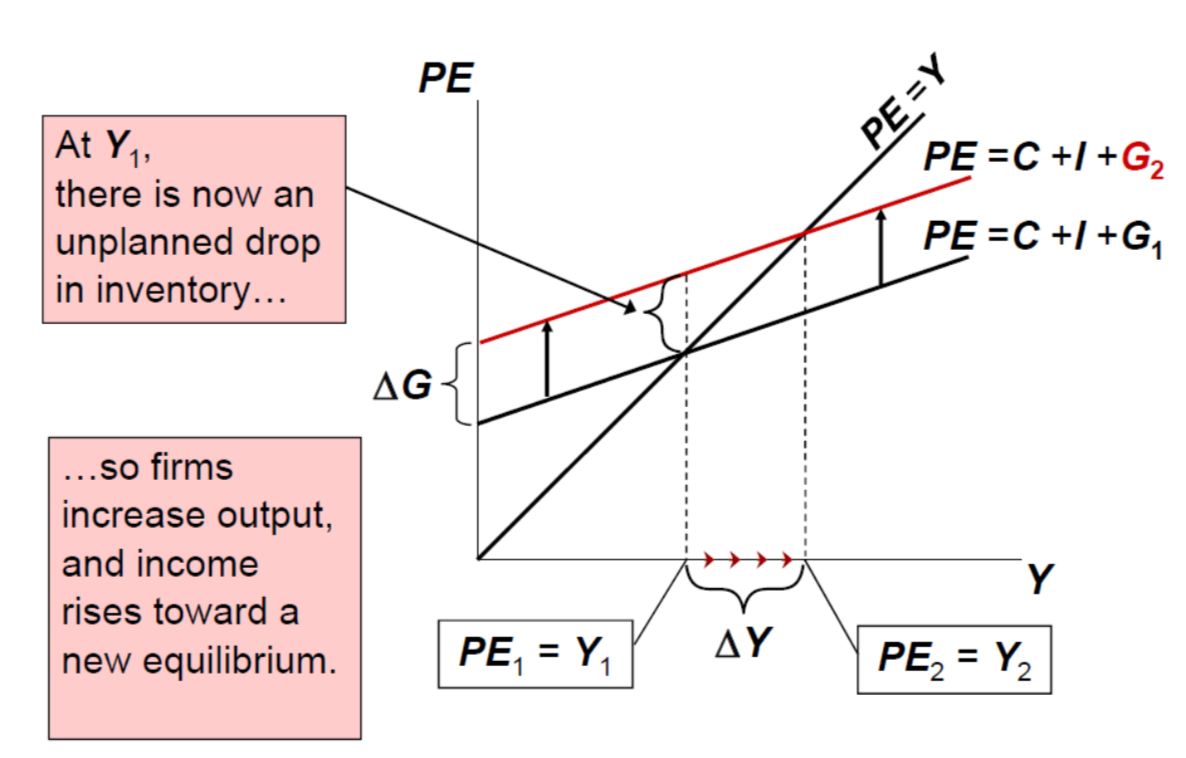
\includegraphics[width=0.6\textwidth]{keynesCross}2
    \caption{The Keynesian Cross: Changing the amount of taxation.}
  \end{center}
\end{figure}

\textbf{THE END!!}

\end{document}

